\chapter{State of the Art}\label{chp:2}
Centuries ago, sailors used to estimate their ships’ positions by using dead reckoning. This method relies on the ship's velocity, previous position and direction of the course in order to estimate the ship's position. At that time, a ship’s course was monitored by a magnetic compass and its velocity calculated by counting the passing knots uniformly spaced on a rope rolled out over the ship’s stern during the time a sandglass emptied  \cite{chp2.1, chp2.2}.  

\par Fortunately, there are various devices and different methods to help to estimate a vehicle's position. For this purpose, there are numerous works are presented in the literature such as different localization techniques with different sensor configuration, data fusion methodologies to find the best estimation and so forth \cite{chp2.3}. 
\par In this chapter, it focuses on the localization of self-driving cars related with the state of the art to become familiar with the concept and discuss possible different sensors and approaches which are used for the localization purpose.

\section{Sensors in Mobile Robotics}
Sensors are key devices for self-driving cars, which enables the vehicle to navigate autonomously in order to accomplish the given tasks. For this reason, self-driving cars must be equipped with several sensors that allow the vehicle to operate themselves by estimating their position relative to their environment \cite{sensor}. Since 2000, a couple quintessential examples of self-driving car's sensor configuration have emerged. Stanley and Boss, the winners of 2005 and 2007, respectively, DARPA urban challenge they showed their vehicle setup in \cite{chp2.4, chp2.5}. Both winners used almost same sensor configuration such as LIDAR, IMU, GPS, and cameras in order to win the competition. It is also important to mention that, our car has also equipped with the similar type of sensor configuration with the winners’ cars as shown in figure \ref{fig:compare_car}.
\par In the following, it describes that what sensors commonly used in the field of autonomous driving.
\begin{figure}[H]
    \centering
    \subfloat[Boss the winner of 2007 DARPA challenge taken from \cite{chp2.5}]{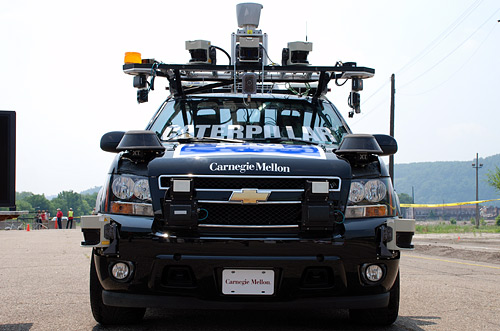
\includegraphics[scale=0.42]{boss}}
    \hfill
    \subfloat[Stanley the winner of 2005 DARPA challenge taken from \cite{chp2.4}]{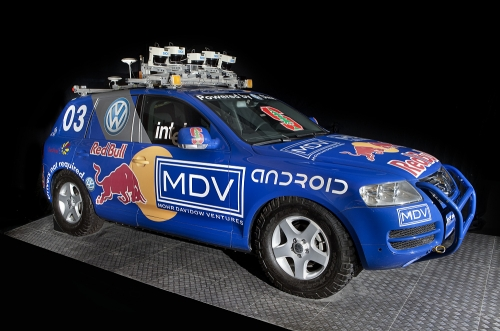
\includegraphics[scale=0.42]{stanley}}
    \caption{Two Examples for Self-driving cars}
    \label{fig:compare_car}
\end{figure}


\subsection*{Rotary encoder}

A rotary encoder is an electro-mechanical device, which reads the angular velocity of wheel in order to estimate the vehicle position \cite{chp2.6}. These sensors are used in a wide range of application even outside of the robotic field, and in most cases they are combined with either steering wheel or gyroscope to calculate wheel odometry \cite{sensor}. However, this technology has a well-known problem, that is wheel slippage \cite{odomja, odometry, odometry1}.

\subsection*{\acrfull{imu}}
\acrshort{imu} is one of the most powerful \acrfull{mems} which is used for tracking velocity and position of any dynamic object \cite{chp2.7}. Since the working principle of IMU relies on the second law of Newton, which is $F=ma$, the velocity and position of any desired object can be easily derived by taking the first and second integral of acceleration, respectively \cite{chp2.7}. Moreover, modern IMUs also provide angular velocity by means of gyroscope. However, since both gyroscope and accelerometer is prone unbounded error due to the sensor bias, therefore, IMU-based localization is subject to drift \cite{chp2.9}. Despite all these facts, IMU is one of the most commonly used sensor in self-driving cars application but it is generally combined with GPS and wheel odometry in order to increase accuracy and robustness of the localization \cite{ACs1,ACs2,chp2.4,chp2.5}.

\subsection*{\acrfull{gps}}
In many robotic application, the \acrshort{gps} is frequently used to estimate the global position of the vehicle \cite{chp2.6}. The advantage of GPS is, it can supply position information independent from the previous position and any weather conditions as long as the area is covered by satellite signals \cite{chp2.6}. However, GPS-based solution, in case of autonomous driving, can be challenging in such a place where GPS might suffer either reflection of signal or poor quality of signal \cite{chp2.10}. Therefore, it is also combined with other sensors as mentioned in \cite{chp2.4,chp2.5,kalman2,kalman6}.

\subsection*{\acrfull{lidar}}
\acrshort{lidar} is a remote sensing method which propagates a bunch of light beam to space and measures reflected light over time in order to calculate a distance of an object and determine its surface \cite{chp2.6}. Thus, LIDAR sensor enables a visualization of the surrounding environments of the vehicle in 3 dimensions in centimeter accuracy-wise. The key application of LIDAR in self-driving cars is to generate a map of an environment for purpose of path planning, obstacle detection, collision avoidance \cite{6D_SLAM,NDT_SLAM,chp2.4, chp2.5}.
\par Taken together, it is clearly understood that sensor fusion technique needs to be used in order to yield a good localization rather than using each sensor individually.

\section{Localization}
In this following sections, different localization techniques are studied as two main topics which are simultaneous localization and mapping and map-based localization.

\subsection*{\acrfull{slam}}
The concept of SLAM is that the mobile robot builds a map of its environment and meantime it estimates its position relative to the map without having any prior information \cite{slam}. 
\par Since the interest of researchers is growing in the autonomous driving field, there are lots of studies are presented to address the SLAM problem. For instance, EKF for SLAM was introduced by Cheeseman et al.\cite{slam1} whose main idea was to estimate robot pose combine with landmark position and to employ EKF to update the pose over a certain time interval. Another example is the Fast-SLAM algorithm, which was introduced by Montemerlo et al.\cite{slam2}, that is based on a particle filter. Its main focus is to deal with the non-linearity of the system whereas EKF-SLAM tries to linearize a nonlinear system which may cause the unreliability, especially for large size map, result in the solution.
\par However, due to concept of the SLAM, it is hard for self-driving cars to build map and use it concurrently for tracking their position at the same time. Therefore to simplify the SLAM problem, another approach which map-based localization (or so-called offline SLAM) is often preferred application for self-driving cars  \cite{slam3}.

\subsection*{Map-Based Localization}
The main idea of this approach is having a prior knowledge about an area for performing localization task in order to estimate and track a position of the vehicle relative to the map. For this purpose, the vehicle is driven manually around an area to acquire sensory data, in our case it was done using by LIDAR, to create map. Afterward, the map is used for localization and navigation \cite{map}. 
\par Since the map of the area is one of the requirements for map-based localization, many different methods can be used to represent the environment. The map can be created by using Graph-SLAM ,which was introduced by Lu and Milos \cite{map3}. They proposed to keep all the scan data together with defined constraint between different poses then apply least square optimization to minimize the error between poses \cite{map4}. Another example is to use scan registration (matching) methods for aligning point sets properly by calculating the transformation between two sets point \cite{icp,3dndt}. 
\par Once the map is created, different localization techniques can be applied. For instance, Monte Carlo localization (MCL) was presented by Dellart et al.\cite{map5}, which is a map based localization relies on a particle filter. An open source version of MCL available in Robot Operating System (ROS)\footnote{\url{http://wiki.ros.org/amcl}} but its application in 2D which means it is not eligible to apply for self-driving cars. Another approach is again to use scan matching methods for localization as mention in by Kato et al. \cite{map1} . They solved localization problem by matching 3D map with LIDAR scan data to find displacement between scan and map at certain time interval. The main idea of this thesis was built on these findings and modified according to the aim of this thesis "Implementation and Evaluation of Localization Methods for Autonomous Cars".

